%************************************************
\chapter{Results}\label{p03:results}
%************************************************
In this chapter, experiments are performed to find the best implementation/settings of the algorithm. As explained in section \ref{p02:session_tracking_read_session}, a wrong value of the "session\_timeout" parameter can produce different and perhaps incorrect results.
First the session timeout for the reading sessions will be determined by trying and analyzing different parameter values. Second, a the session timeout for the exercise sessions will be determined.

\section{Reading session experiments}
The reading session tracking is the most complex to model, because there are multiple internal and external variables to consider. First, we must define what actions are relevant to detect, in order to consider them as part of the learning process, and which ones are not (\Ie\ the user trying to game the system). Second, with the events already defined, we must determine how much time can pass between them, which is still part of the same reading/learning session.

User actions were classified as follows:
\begin{itemize}
	\item Opening
		\begin{itemize}
			\item Article focused
			\item Open article
			\item Open starred article
		\end{itemize}
	
	\item Interaction
		\begin{itemize}
			\item Change orientation
			\item Open alter menu
			\item Close alter menu
			\item Send suggestion
			\item Speak text
			\item Translate text
			\item Undo text translation
			\item Scroll
		\end{itemize}
	
	\item Closing
		\begin{itemize}
			\item Article closed
			\item Articles requested from Zeeguu
		\end{itemize}
\end{itemize}


\subsection{Baseline}
For the baseline an arbitary value of 5 minutes for the \textbf{session\_timeout} was used.

By observing the total reading time by user, we can see that the highest value is 2788 minutes (almost 2 days). By analyzing the daily activity for a specific user, we find long reading sessions spanning up to 1:20 hours long. Figure \ref{fig:visualizations_1st_iteration} show these results.

\begin{figure}[bth]
	\myfloatalign
	\subfloat[Total read time by user]
	{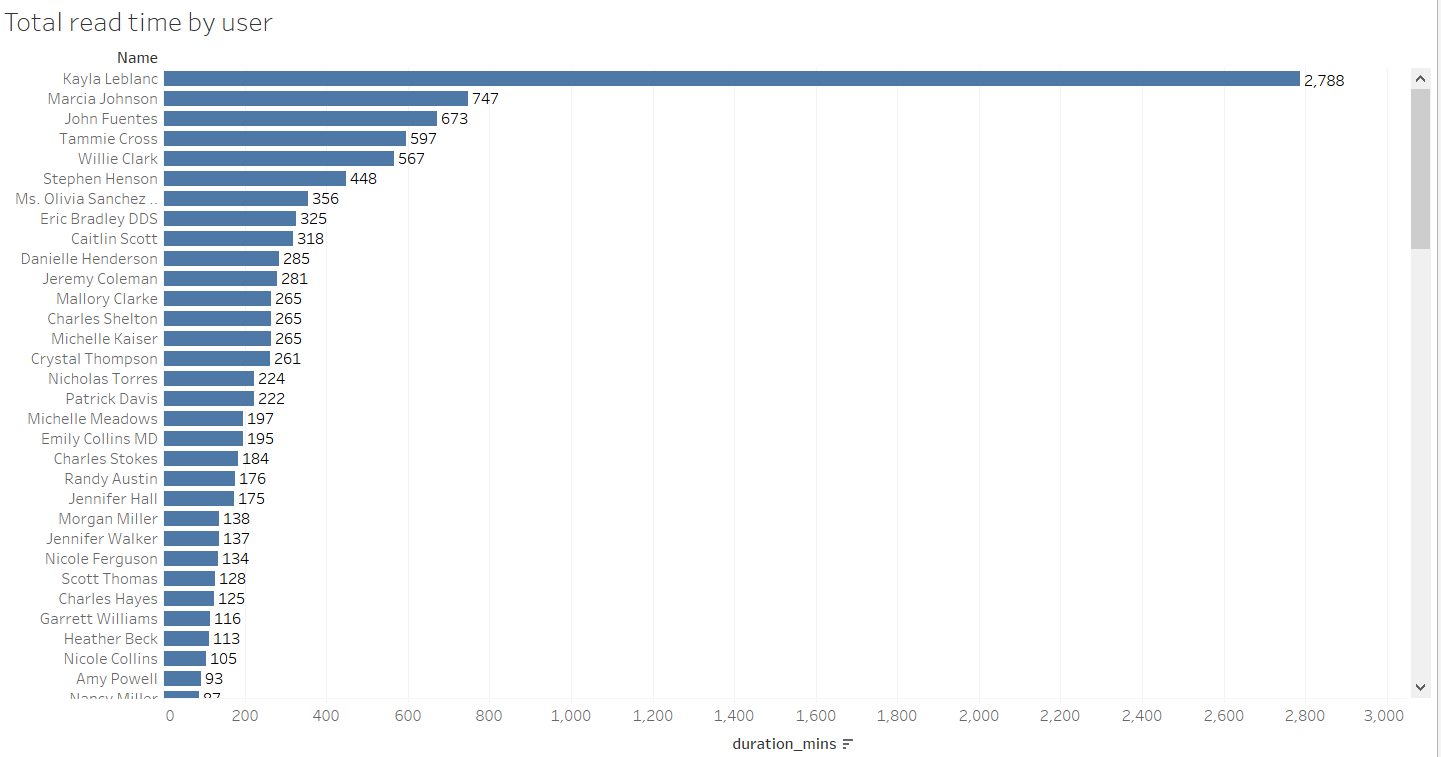
\includegraphics[width=1\linewidth]{gfx/total_read_time_by_user_5min}\label{fig:total_read_time_5min_no_scroll}} \quad 
	\subfloat[Daily activity timeline]
	{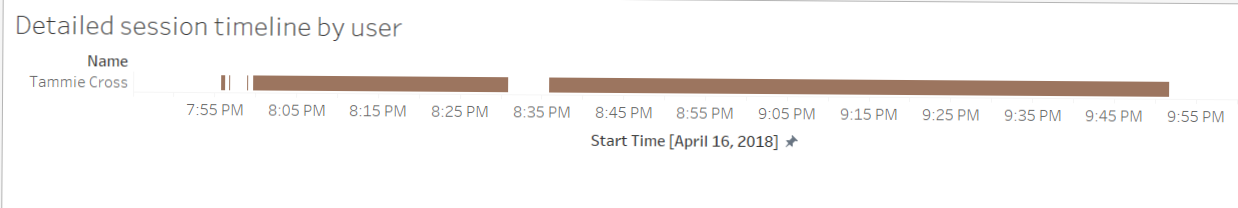
\includegraphics[width=1\linewidth]{gfx/detailed_session_timeline_by_user_5min_no_scroll}\label{fig:detailed_session_timeline_by_user_5min_no_scroll}} \quad
	\caption{Reading session visualizations for session\_timeout of 5 minutes.}\label{fig:visualizations_1st_iteration}
\end{figure}


\subsection{Improving the baseline}
Using the previous settings as a baseline, the next idea was to reduce the value of session\_timeout, because the additional time benefit of 5 minutes might be too much grace time for a user reading without doing any action. Scrolling events are helpful to detect more frequent activity, but they can be overwhelming for the web server and the database, for that reason, the web server callback was limited to maximum 1 call per minute. This implies that the minimum timeout value should be at least 1 minute.

Sessions were computed using different parameters for the session\_timeout, and the maximum idle time between user actions inside a session was plotted (Figure \ref{fig:idle_time_comparison}).

\begin{figure}[bth]
	\myfloatalign
	\subfloat[1 min]
	{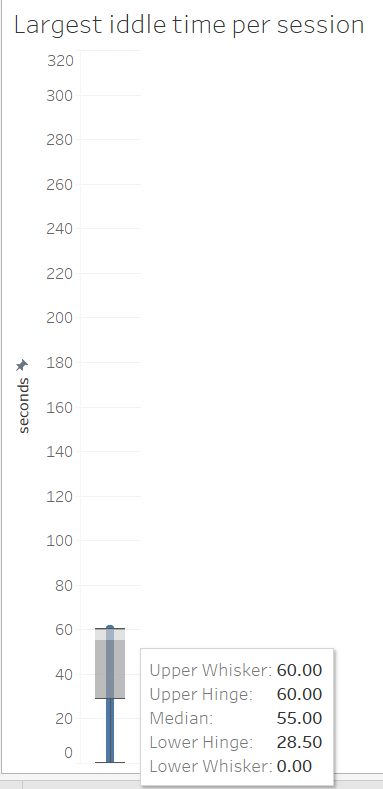
\includegraphics[width=0.19\linewidth]{gfx/largest_iddle_time_1min_timeout}\label{fig:largest_iddle_time_1min_timeout}}  
	\subfloat[2 min]
	{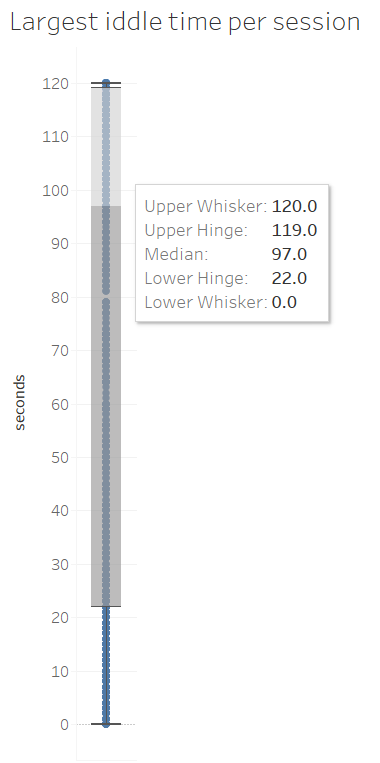
\includegraphics[width=0.19\linewidth]{gfx/largest_iddle_time_2min_timeout}\label{fig:largest_iddle_time_2min_timeout}} 
	\subfloat[3 min]
	{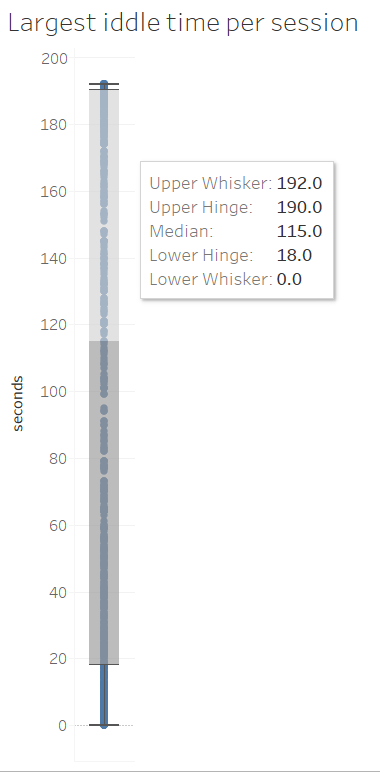
\includegraphics[width=0.19\linewidth]{gfx/largest_iddle_time_3o2min_timeout}\label{fig:largest_iddle_time_3o2min_timeout}}
	\subfloat[4 min]
	{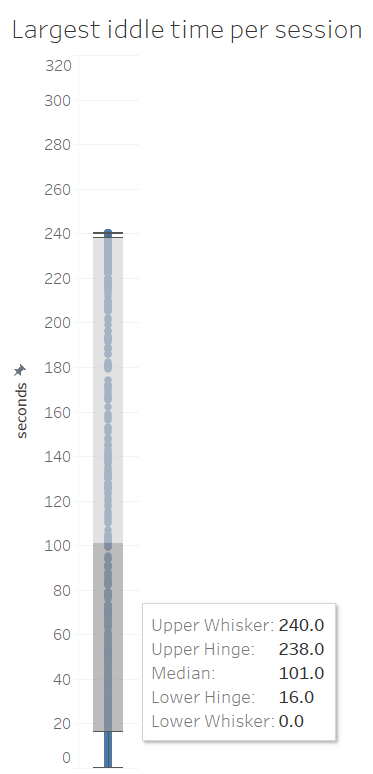
\includegraphics[width=0.19\linewidth]{gfx/largest_iddle_time_4min_timeout}\label{fig:largest_iddle_time_4min_timeout}} 
	\subfloat[5 min]
	{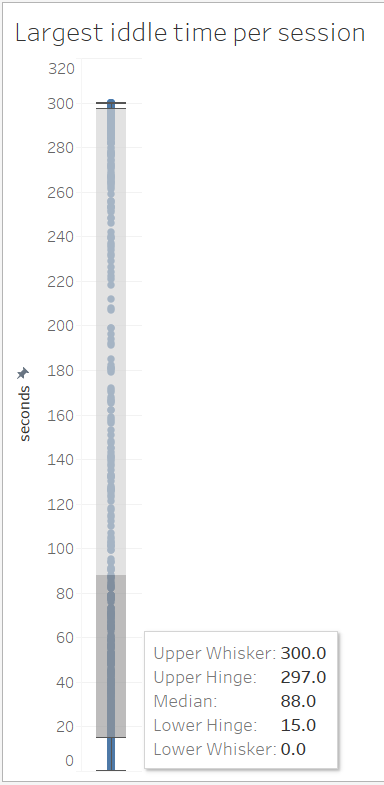
\includegraphics[width=0.19\linewidth]{gfx/largest_iddle_time_5min_timeout}\label{fig:largest_iddle_time_5min_timeout_v2}} \quad
	
	\caption{Box plot of maximum idle time per session, for distinct session timeout values}\label{fig:idle_time_comparison}
\end{figure}

We can observe that the median value fluctuates between 90 and 120 seconds (as shown in Table \ref{tb:table_median_value}). By taking this value into account and some empirical measures, the value of the timeout was set to 2 minutes. 

The upper hinge, however, increases as the timeout value do. This is because small sessions are stitched together, therefore moving the value upwards.

\begin{table}[htb]
	\begin{tabularx}
		{\textwidth}{Xllll}\toprule
		\tableheadline{Timeout value (min)} & 
		\tableheadline{Median (sec)} &
		\tableheadline{Upper hinge(sec)} \\ 
		\midrule 
		1 & 55 & 60 \\ 
		\hline 
		2 & 97 & 119 \\ 
		\hline
		3.2 & 115 & 190\\ 
		\hline 
		4 & 101 & 238\\ 
		\hline 
		5 & 88 & 297\\ 
		\hline 
	\end{tabularx} 
	\caption{Maximum idle time statistics with different session timeout values}\label{tb:table_median_value}
\end{table}

By comparing the total time per user between the baseline and the final settings (figure \ref{fig:total_time_comparison}), we can observe that a reduction of almost 300\% in the total time per user was achieved. This means that the session\_timeout value has a huge impact, specially when comparing over long periods of time.

\begin{figure}[!htb]
	\myfloatalign
	\subfloat[Baseline (5 minutes)]
	{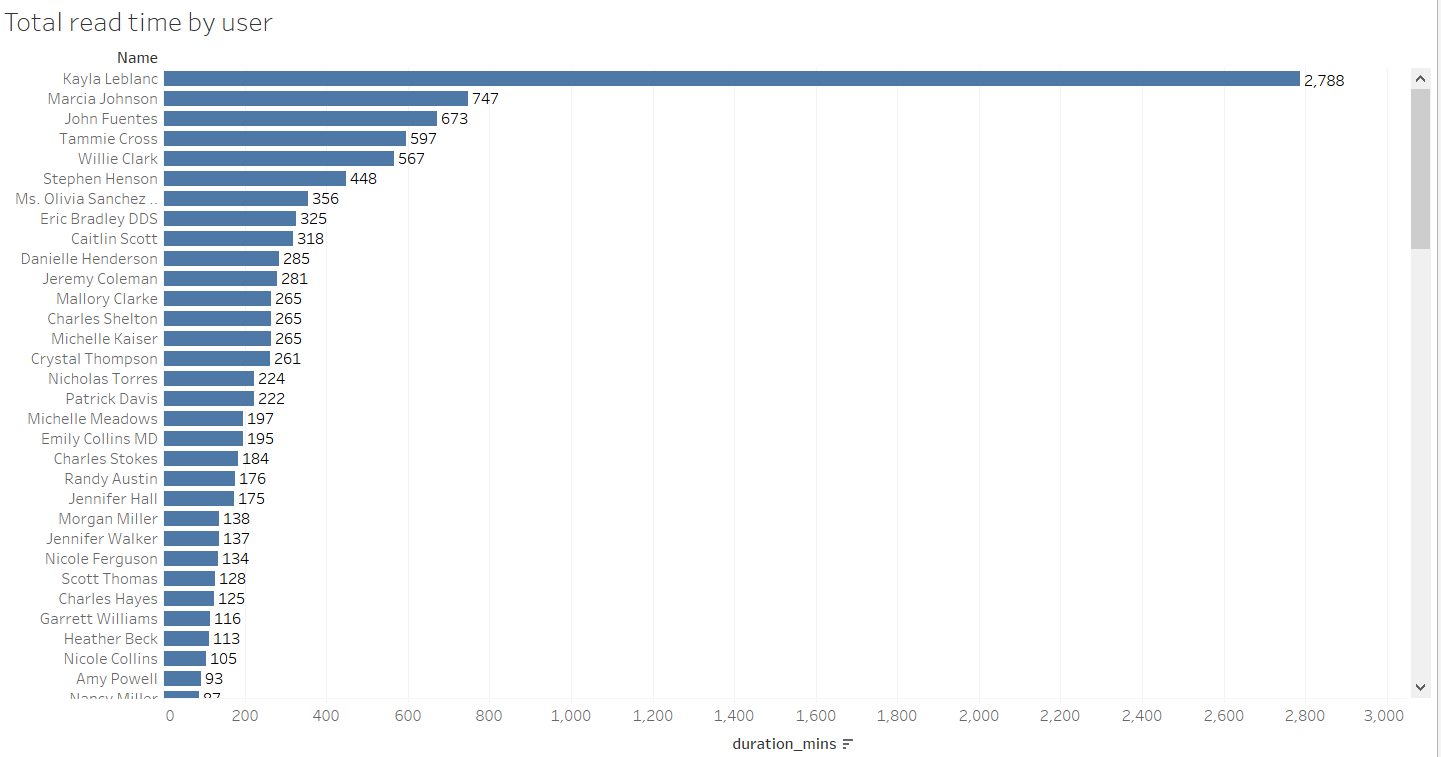
\includegraphics[width=1\linewidth]{gfx/total_read_time_by_user_5min}\label{fig:total_read_time_by_user_5min}} \quad 
	\subfloat[Final settings (2 minutes)]
	{
	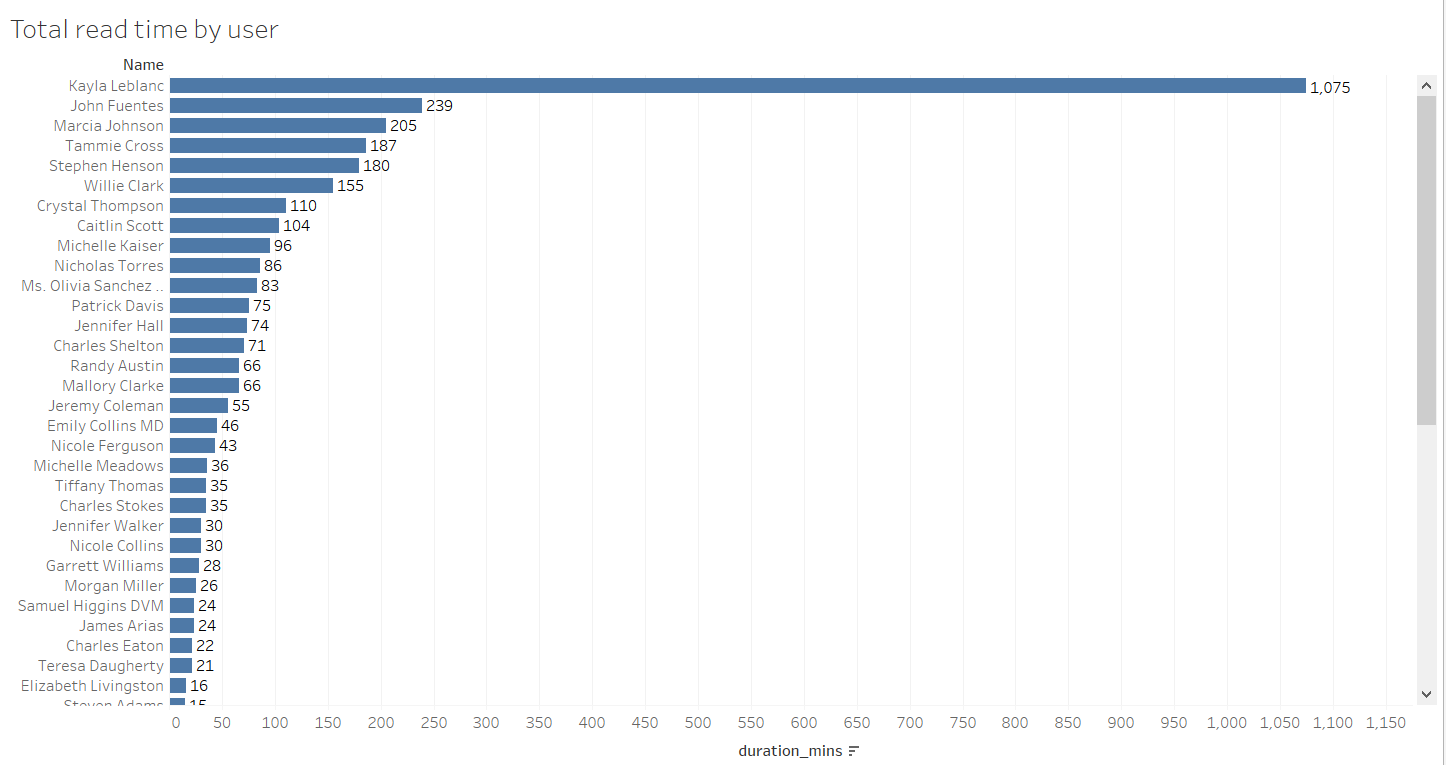
\includegraphics[width=1\linewidth]{gfx/total_read_time_by_user_2min}\label{fig:total_read_time_by_user_2min}} \\
	\caption{Total time improvement comparison}\label{fig:total_time_comparison}
\end{figure}

Finally, for the detailed activity, a big change is observed, in Figure \ref{fig:detailed_session_5min}, we observe roughly two smooth reading sessions, which later, with a finer session detection gets split into smaller reading sessions (Figure \ref{fig:detailed_session_2min}). This suggests that we correctly detected the user's gap of attentions, therefore a more precise session time was measured.

\begin{figure}[!htb]
	\myfloatalign
	\subfloat[Baseline (5 minutes)]
	{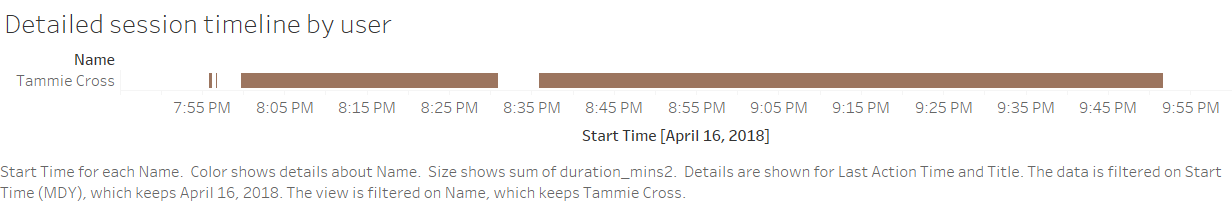
\includegraphics[width=1\linewidth]{gfx/detailed_session_timeline_by_user_5min}\label{fig:detailed_session_5min}} \quad 
		
	\subfloat[Final settings (2 minutes)]
	{
	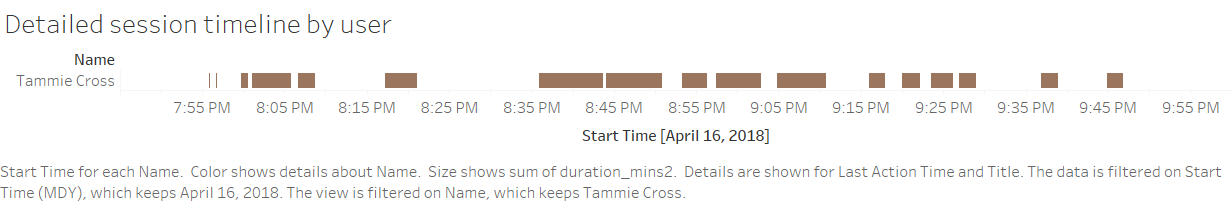
\includegraphics[width=1\linewidth]{gfx/detailed_session_timeline_by_user_2min}\label{fig:detailed_session_2min}} \\
	\caption{Low level session tracking time line}\label{fig:detailed_session_comparison}
\end{figure}


\subsection{Validation}
Before the implementation of the session tracking, students manually reported the time spent reading in Zeeguu. Therefore a useful validation of the computed session tracking is against the time reported by students.

Table \ref{tb:comparison_read_time} shows the comparison between the reported time and the computed total time using session tracking for a period of six months.

There is a clear difference between both times. The reported time is 4 times bigger than the computed time.

The validation against the time reported by students did not match as expected, the most probable reason is that students rounded up to the next half hour while generating the reports because that is their unit of measure. 

\begin{table}[!htb]
	\tiny
	\resizebox{\textwidth}{!}{
	\begin{tabularx}
		{\textwidth}{XXXXX}\toprule
		\tableheadline{Student} & 
		\tableheadline{Read time} &
		\tableheadline{Exercise time} &
		\tableheadline{Total detected time} &
		\tableheadline{Reported time} \\ 
		\midrule 
		Student 1
		  & 59 min
		  & 1 hour 24 min
		  & 2 hours 23 min
		  & 10 hours
		   \\ 
		\hline 
		Student 2
		  & 44 min
		  & 0 min
		  & 44 min
		  & 2 hour 30 min
		   \\ 
		\hline
		Student 3
		  & 54 min
		  & 2.8 min
		  & 56.8 min
		  & 4 hours
		  \\ 
		\hline 
	\end{tabularx} 
}
	\caption{Comparison of working time reported by students vs the time computed by the algorithm (using a timeout value of 2 minutes for reading sessions and 21 seconds for exercise sessions)}\label{tb:comparison_read_time}
\end{table}

\section{Exercise session experiments}
For the exercise sessions, the implementation is simple. Exercise user events were classified as follows:

\begin{itemize}
	\item Opening
		\begin{itemize}
			\item Opening exercise
		\end{itemize}
		
	\item Interaction
		\begin{itemize}
			\item Answer exercise
			\item Asking for a hint
		\end{itemize}
\end{itemize}

Given that answering marks the end of an exercise, no additional "closing" actions were used. Therefore the exercise session is finalized whenever the timeout expires. However, in contrast with the reading session, for exercise sessions no grace time is given, meaning that the time of the end of the session is marked by the last completed exercise, and not when the timeout expires.

For the exercises, we know that they are short and quick activities, which take only a couple of second to provide an answer. Therefore the timeout must be much smaller than for reading.

In this case, the time between the exercise opening and the answering is computed by a timer. Therefore by utilizing a descriptive analysis of the answering time (box plot in Figure \ref{fig:exercise_solving_speed}). The obtained results are 6, 10 and 21 seconds, which represent the median, upper hinge and upper whisker. These metrics correspond the 50\%, 75\% and 100\%, of the sessions at hand. 

\begin{figure}[bth]
	\centering
	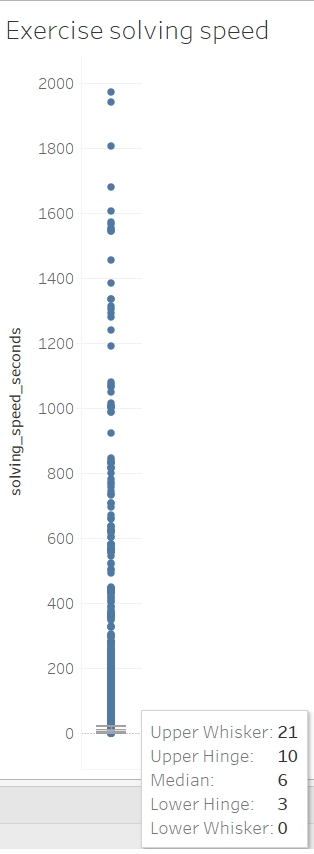
\includegraphics[width=0.2\linewidth]{gfx/exercise_solving_speed}
	\caption{Exercise solving speed boxplot}\label{fig:exercise_solving_speed}
\end{figure}

Given that the tracked time window is so small, a final setup of no grace time but using the upper whisker value (21 seconds) is chosen.


